\section{Background}

\subsection{Classical Prisoner's Dilemma}

The prisoner's dilemma is a two-player non-zero-sum game involving the actions cooperate $(C)$ and defect $(D)$. The payoff ordering satisfies

\begin{equation}
	T > R > P > S,
\end{equation}

where $T$ denotes the temptation payoff, $R$ the reward for mutual cooperation, $P$ the punishment for mutual defection, and $S$ the sucker's payoff.

A common numerical assignment is

\begin{equation}
	T = 3,\quad R = 2,\quad P = 1,\quad S = 0.
\end{equation}

\begin{table}[H]
	\centering
	\caption{Payoff matrix for Bonnie and Clyde.}
	\label{tab:prisoners}
	
	\renewcommand{\arraystretch}{2.5}
	\setlength{\tabcolsep}{8pt}
	
	\begin{tabular}{c|c|c}
		& \shortstack{Clyde\\cooperates}
		& \shortstack{Clyde\\defects} \\
		\hline
		\shortstack{Bonnie\\cooperates}
		& $(R,R)$
		& $(S,T)$ \\
		\hline
		\shortstack{Bonnie\\defects}
		& $(T,S)$
		& $(P,P)$
	\end{tabular}
\end{table}

Although $(C,C)$ is Pareto superior, the Nash equilibrium is $(D,D)$ because unilateral deviation from cooperation increases individual payoff.

\subsection{Non-Zero-Sum Symmetric Games}

The prisoner's dilemma is one example of a non-zero-sum symmetric game~\cite{nash}. Another classical example is the game of chicken, in which players benefit from avoiding mutual conflict while attempting to avoid unilateral disadvantage. Unlike the prisoner's dilemma, chicken admits multiple Nash equilibria and emphasizes strategic coordination rather than dominant-strategy defection~\cite{jankowski}.

\begin{table}[H]
	\centering
	\caption{Payoff matrix for the game of chicken played by players $P_1$ and $P_2$.}
	\label{tab:chicken}
	
	\renewcommand{\arraystretch}{2}
	\setlength{\tabcolsep}{8pt}
	
	\begin{tabular}{c|c|c}
		& $P_2$ swerves & $P_2$ straight \\
		\hline
		$P_1$ swerves  & $(0,0)$ & $(1,-1)$ \\
		\hline
		$P_1$ straight & $(-1,1)$ & $(-1000,-1000)$
	\end{tabular}
\end{table}

These examples illustrate how equilibrium structure may vary substantially across strategic environments, motivating the study of how quantum correlations alter equilibrium behavior in non-cooperative games.

\subsection{Nash Equilibrium}

A strategy profile $s^*$ is a Nash equilibrium if no player can improve payoff by changing strategy alone:

\begin{equation}
	u_i(s_i^*, s_{-i}^*)
	\ge
	u_i(s_i, s_{-i}^*)
\end{equation}

for all admissible strategies $s_i$.

\subsection{Quantum Computing Concepts}

This analysis relies on standard quantum-mechanical principles including superposition, measurement, and entanglement.

\paragraph{Superposition.}

A qubit may exist in a linear combination of basis states:

\begin{equation}
	|\psi\rangle = \alpha |0\rangle + \beta |1\rangle,
\end{equation}

where

\begin{equation}
	|\alpha|^2 + |\beta|^2 = 1.
\end{equation}

\begin{figure}[H]
	\centering
	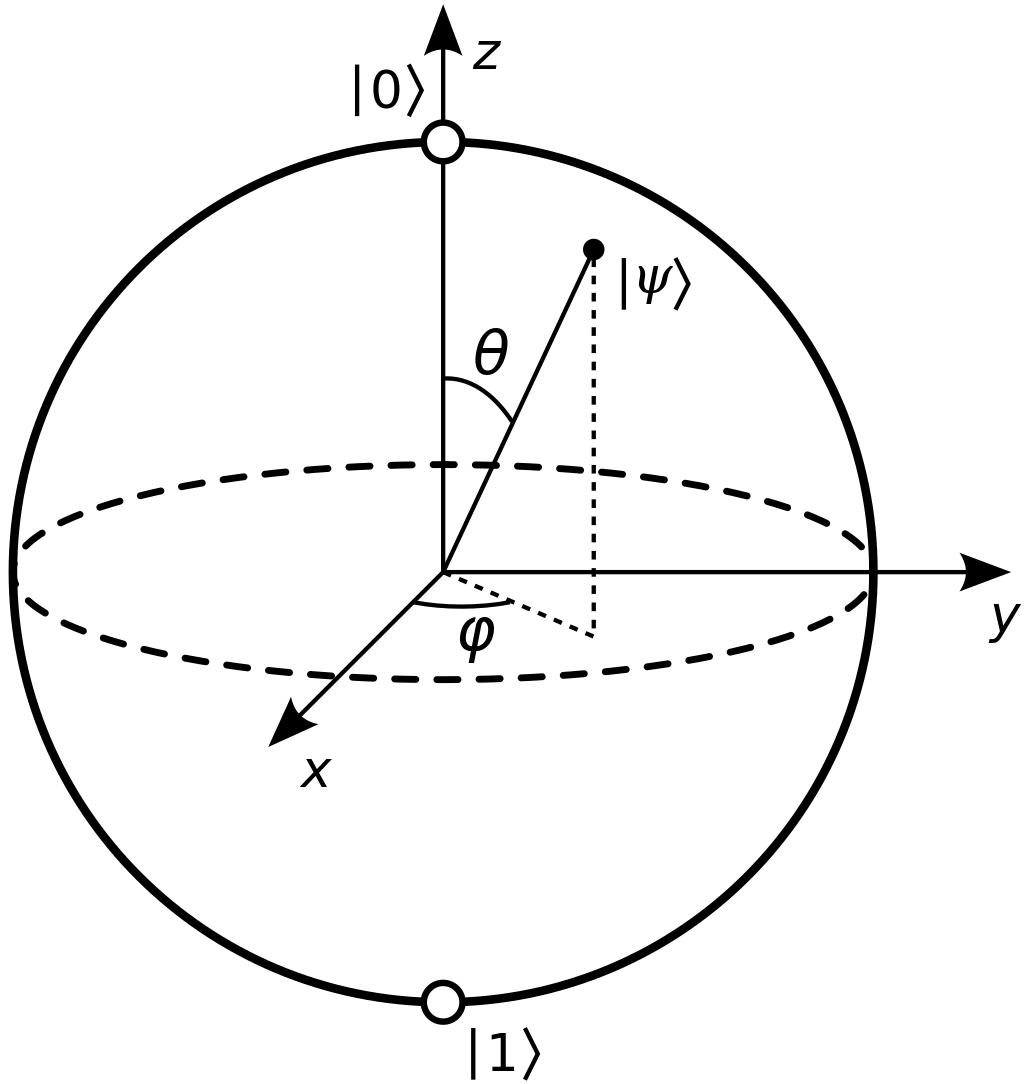
\includegraphics[scale=0.1]{tikz/bloch.png}
	\caption{Bloch sphere representation of a qubit state.}
	\label{fig:bloch}
\end{figure}

\paragraph{Measurement.}

Measurement collapses a quantum state probabilistically. The outcomes $|0\rangle$ and $|1\rangle$ occur with probabilities $|\alpha|^2$ and $|\beta|^2$ respectively.

\begin{figure}[H]
	\centering
	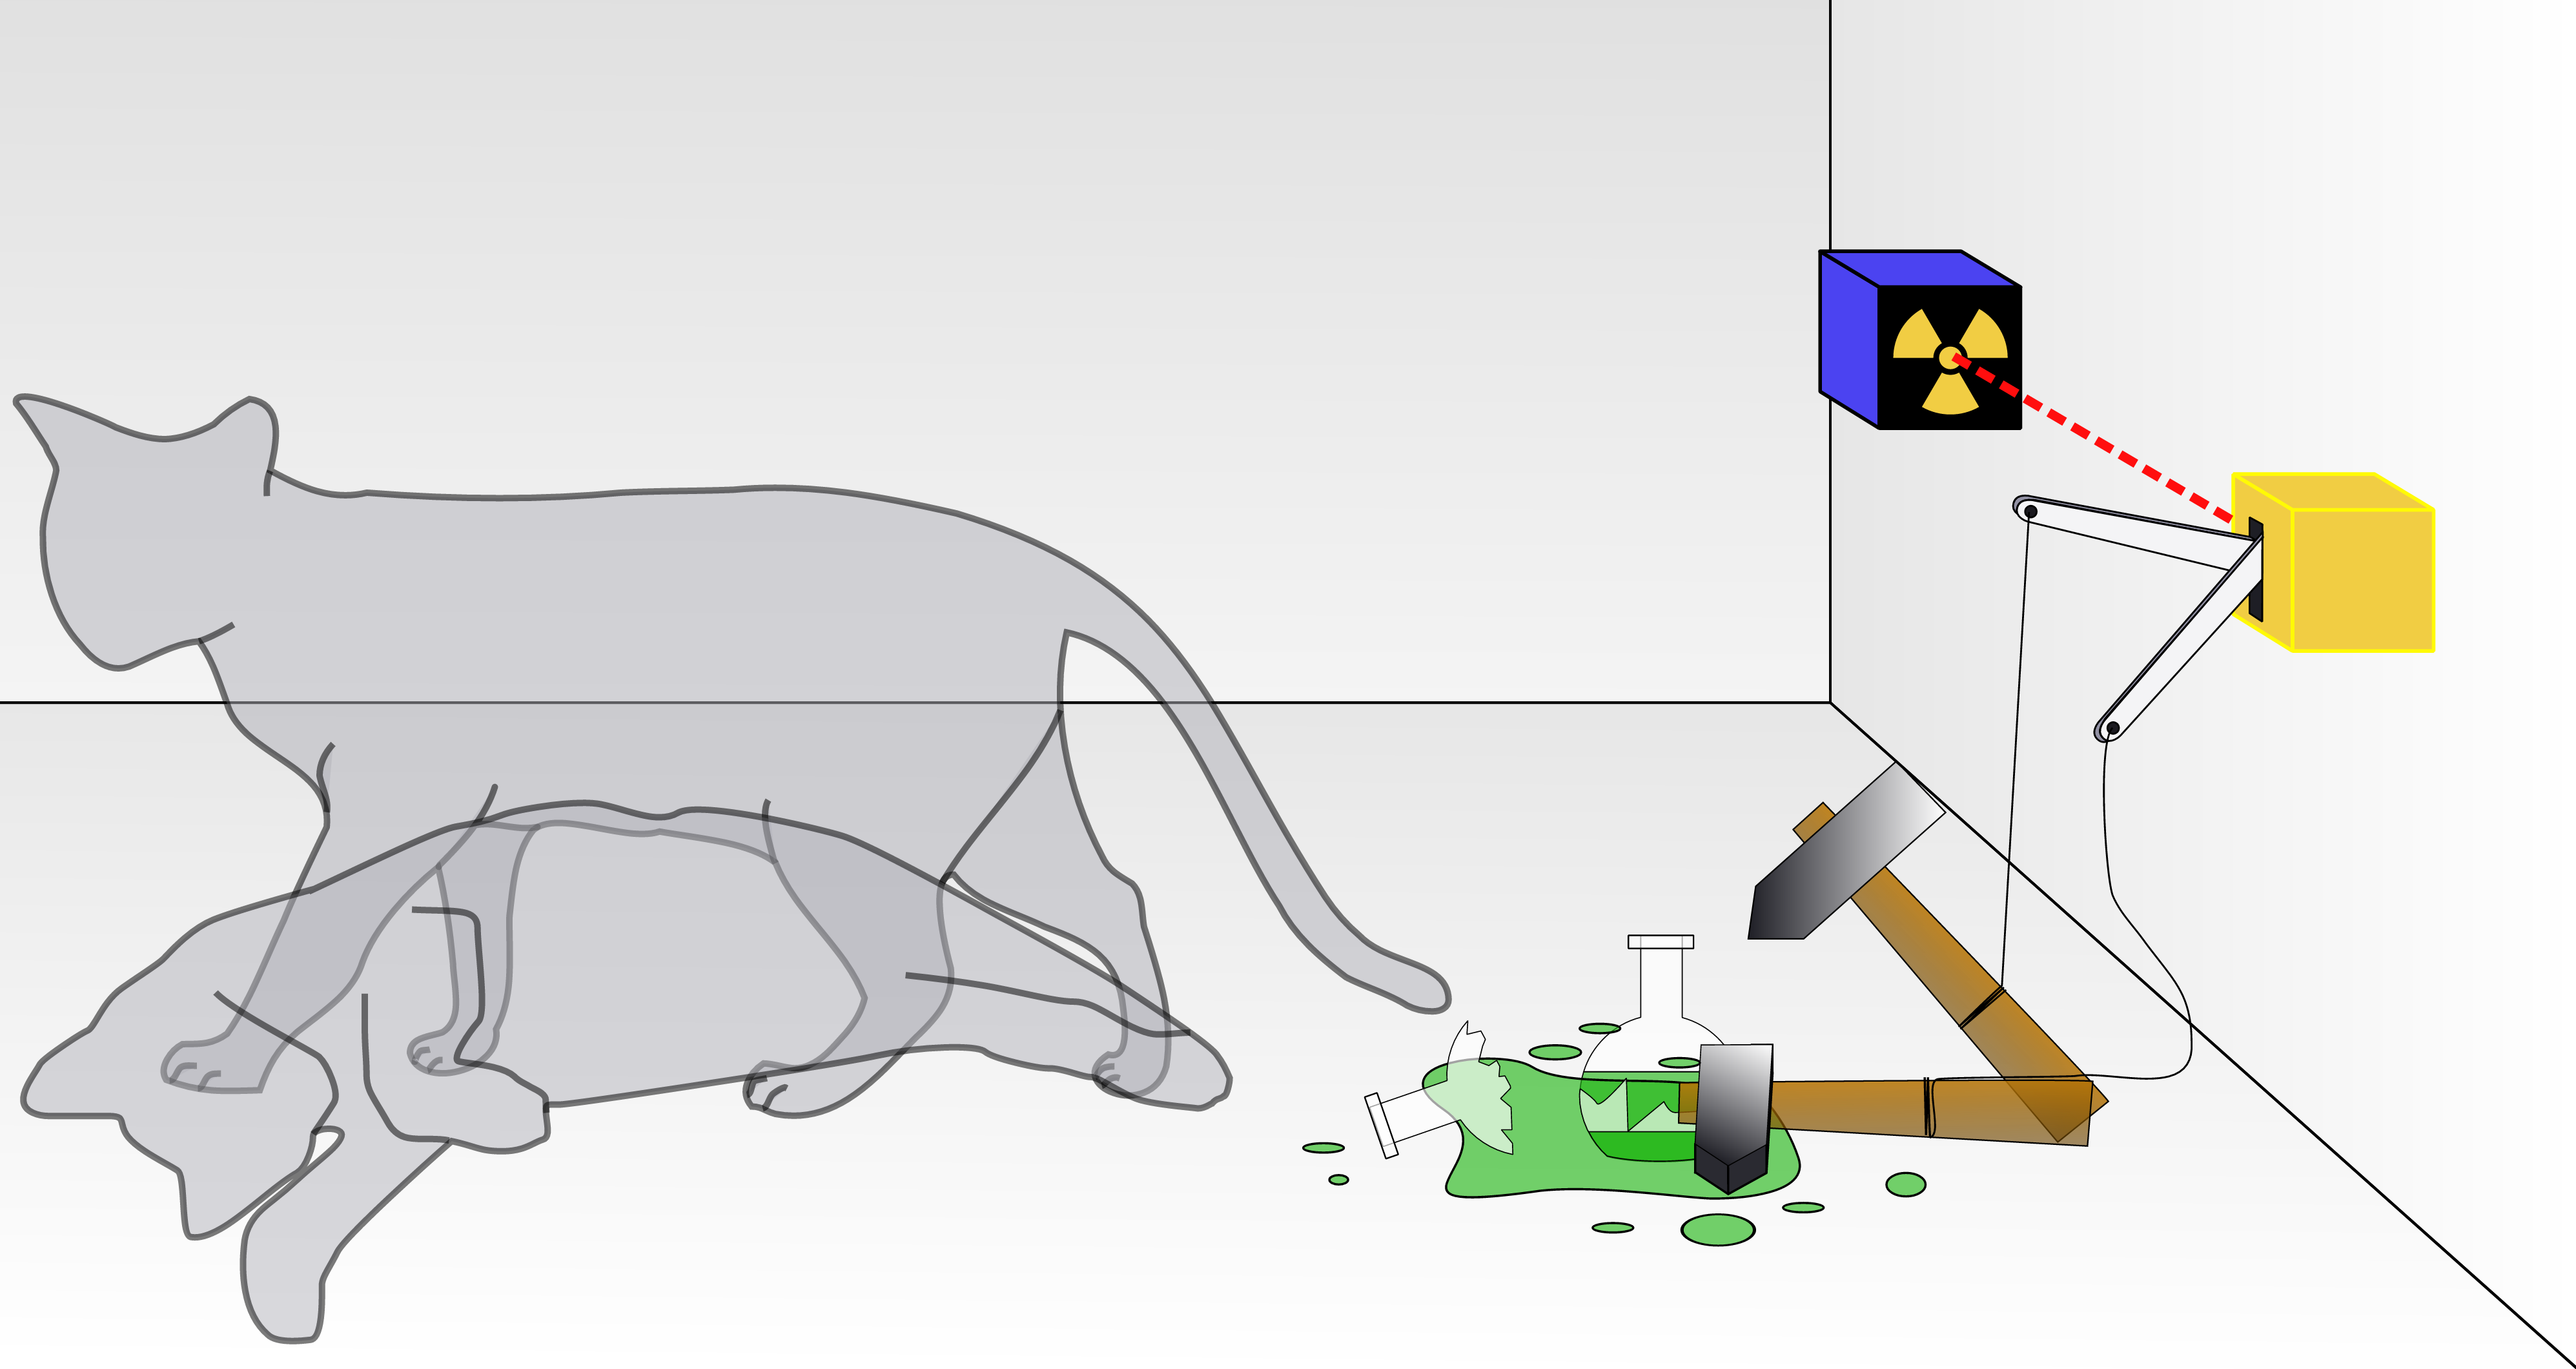
\includegraphics[scale=0.04]{tikz/Schrodingers_cat.png}
	\caption{Illustration of Schrödinger's cat thought experiment.}
	\label{fig:schrodinger}
\end{figure}

\paragraph{Entanglement.}

Two systems are entangled when their joint state cannot be decomposed into independent tensor products:

\begin{equation}
	|\psi\rangle \neq |\psi_A\rangle \otimes |\psi_B\rangle.
\end{equation}

Entanglement creates correlations that may not be reproducible through classical independent randomization.